% THIS DOCUMENT IS FOLLOWS THE VOLERE TEMPLATE BY Suzanne Robertson and James Robertson
% ONLY THE SECTION HEADINGS ARE PROVIDED
%
% Initial draft from https://github.com/Dieblich/volere
%
% Risks are removed because they are covered by the Hazard Analysis
\documentclass[12pt]{article}
\usepackage{graphicx}
\usepackage{booktabs}
\usepackage{tabularx}
\usepackage{hyperref}
\hypersetup{
    bookmarks=true,         % show bookmarks bar?
      colorlinks=true,      % false: boxed links; true: colored links
    linkcolor=red,          % color of internal links (change box color with linkbordercolor)
    citecolor=green,        % color of links to bibliography
    filecolor=magenta,      % color of file links
    urlcolor=cyan           % color of external links
}

\newcommand{\lips}{\textit{Insert your content here.}}

%% Comments

\usepackage{color}

\newif\ifcomments\commentstrue %displays comments
%\newif\ifcomments\commentsfalse %so that comments do not display

\ifcomments
\newcommand{\authornote}[3]{\textcolor{#1}{[#3 ---#2]}}
\newcommand{\todo}[1]{\textcolor{red}{[TODO: #1]}}
\else
\newcommand{\authornote}[3]{}
\newcommand{\todo}[1]{}
\fi

\newcommand{\wss}[1]{\authornote{magenta}{SS}{#1}} 
\newcommand{\plt}[1]{\authornote{cyan}{TPLT}{#1}} %For explanation of the template
\newcommand{\an}[1]{\authornote{cyan}{Author}{#1}}

%% Common Parts

\newcommand{\progname}{SFWRENG 4G06 - Capstone Design Process}
\newcommand{\authname}{\textbf{Team 17, DomainX} \\
\\ Awurama Nyarko
\\ Haniye Hamidizadeh
\\ Fei Xie
\\ Ghena Hatoum             
}
\usepackage{hyperref}
    \hypersetup{colorlinks=true, linkcolor=blue, citecolor=blue, filecolor=blue,
                urlcolor=blue, unicode=false}
    \urlstyle{same}
                                


\begin{document}

\title{Software Requirements Specification for \progname: subtitle describing software} 
\author{\authname}
\date{\today}
	
\maketitle

\pagenumbering{roman}
\begin{table}[hp]
\caption{Revision History} \label{TblRevisionHistory}
\begin{tabularx}{\textwidth}{llX}
\toprule
\textbf{Date} & \textbf{Developer(s)} & \textbf{Change}\\
\midrule
October 6, 2025 & Fei Xie & First Draft of Sections: Cost to Ideas for Solution\\
Date2 & Name(s) & Description of changes\\
... & ... & ...\\
\bottomrule
\end{tabularx}
\end{table}

~\newpage

\tableofcontents

~\newpage
\section{Purpose of the Project}
\subsection{User Business}
\lips
\subsection{Goals of the Project}
\lips
\section{Stakeholders}
\subsection{Client}
\lips
\subsection{Customer}
\lips
\subsection{Other Stakeholders}
\lips
\subsection{Hands-On Users of the Project}
\lips
\subsection{Personas}
\lips
\subsection{Priorities Assigned to Users}
\lips
\subsection{User Participation}
\lips
\subsection{Maintenance Users and Service Technicians}
\lips

\section{Mandated Constraints}
\subsection{Solution Constraints}
\lips
\subsection{Implementation Environment of the Current System}
\lips
\subsection{Partner or Collaborative Applications}
\lips
\subsection{Off-the-Shelf Software}
\lips
\subsection{Anticipated Workplace Environment}
\lips
\subsection{Schedule Constraints}
\lips
\subsection{Budget Constraints}
\lips
\subsection{Enterprise Constraints}
\lips

\section{Naming Conventions and Terminology}
\subsection{Glossary of All Terms, Including Acronyms, Used by Stakeholders
involved in the Project}
\lips

\section{Relevant Facts And Assumptions}
\subsection{Relevant Facts}
\lips
\subsection{Business Rules}
\lips
\subsection{Assumptions}
\lips

\section{The Scope of the Work}
\subsection{The Current Situation}
\lips
\subsection{The Context of the Work}
\lips
\subsection{Work Partitioning}
\lips
\subsection{Specifying a Business Use Case (BUC)}
\lips

\section{Business Data Model and Data Dictionary}
\subsection{Business Data Model}
\lips
\subsection{Data Dictionary}
\lips

\section{The Scope of the Product}
\subsection{Product Boundary}
\lips
\subsection{Product Use Case Table}
\lips
\subsection{Individual Product Use Cases (PUC's)}
\lips

\section{Functional Requirements}
\subsection{Functional Requirements}
\lips

\section{Look and Feel Requirements}
\subsection{Appearance Requirements}
\lips
\subsection{Style Requirements}
\lips

\section{Usability and Humanity Requirements}
\subsection{Ease of Use Requirements}
\lips
\subsection{Personalization and Internationalization Requirements}
\lips
\subsection{Learning Requirements}
\lips
\subsection{Understandability and Politeness Requirements}
\lips
\subsection{Accessibility Requirements}
\lips

\section{Performance Requirements}
\subsection{Speed and Latency Requirements}
\lips
\subsection{Safety-Critical Requirements}
\lips
\subsection{Precision or Accuracy Requirements}
\lips
\subsection{Robustness or Fault-Tolerance Requirements}
\lips
\subsection{Capacity Requirements}
\lips
\subsection{Scalability or Extensibility Requirements}
\lips
\subsection{Longevity Requirements}
\lips

\section{Operational and Environmental Requirements}
\subsection{Expected Physical Environment}
\lips
\subsection{Wider Environment Requirements}
\lips
\subsection{Requirements for Interfacing with Adjacent Systems}
\lips
\subsection{Productization Requirements}
\lips
\subsection{Release Requirements}
\lips

\section{Maintainability and Support Requirements}
\subsection{Maintenance Requirements}
\lips
\subsection{Supportability Requirements}
\lips
\subsection{Adaptability Requirements}
\lips

\section{Security Requirements}
\subsection{Access Requirements}
\lips
\subsection{Integrity Requirements}
\lips
\subsection{Privacy Requirements}
\lips
\subsection{Audit Requirements}
\lips
\subsection{Immunity Requirements}
\lips

\section{Cultural Requirements}
\subsection{Cultural Requirements}
\lips

\section{Compliance Requirements}
\subsection{Legal Requirements}
\lips
\subsection{Standards Compliance Requirements}
\lips

\section{Open Issues}

The following unresolved items could materially affect the design, deployment,
or operation of the NNL Assessment Tool. The issues in
Table~\ref{tab:open-issues} will be tracked until closure to reduce delivery
risk and surprises in later phases.

\begin{table}[hp]
\caption{Open issues to track and resolve} \label{tab:open-issues}
\begin{tabularx}{\textwidth}{p{1.6cm}X X X X p{2.1cm}}
\toprule
\textbf{Issue \#} & \textbf{Summary} & \textbf{Cross-Reference} &
\textbf{Stakeholders} & \textbf{Action Required} & \textbf{Status} \\
\midrule
OI-01 & Finalize hosting environment for the tool (e.g., internal server or
university-managed cloud). & Operational and Environmental Requirements &
CAS Supervisor, Infrastructure Team & Confirm approved infrastructure with IT &
Pending \\
\addlinespace[0.3em]
OI-02 & Confirm the final list of neural network libraries to include in the
tool’s database (based on domain-expert review). & Scope of the Work &
Research Subteam, Domain Expert & Schedule and complete review with domain
expert & Pending \\
\addlinespace[0.3em]
OI-03 & Select user interface (UI) framework and visualization library
(e.g., React with Chart.js vs.\ D3). & Functional Requirements &
Development Team & Evaluate options and record decision & In progress \\
\addlinespace[0.3em]
OI-04 & Decide Excel integration level (import/export only or live
synchronization with spreadsheets). & Functional Requirements & Research
Subteam, Developers & Define use cases and confirm feasibility & Pending \\
\addlinespace[0.3em]
OI-05 & Choose authentication method: McMaster single sign-on (SSO) versus
custom login. & Security Requirements; Operational and Environmental
Requirements & CAS Supervisor, Development Team & Meet with IT to assess SSO
feasibility & Pending \\
\addlinespace[0.3em]
OI-06 & Confirm data storage architecture (e.g., structured query language
(SQL) database versus alternative storage). & Operational and Environmental
Requirements & Developers, Infrastructure Team & Evaluate options and finalize
design & Pending \\
\bottomrule
\end{tabularx}
\end{table}


\section{Off-the-Shelf Solutions}

This section identifies existing tools, software, and components that could be leveraged to reduce development time and cost for the Neural Network Libraries (NNL) Assessment Tool. It outlines reusable libraries and products that can be legally copied or adapted to accelerate development and ensure maintainability.

The goal is to reuse proven, reliable components and avoid reinventing existing functionality, thereby optimizing development effort and leveraging established best practices.

\subsection{Ready-Made Products}

Several existing platforms provide partial functionality aligned with the tool’s goals, particularly in data visualization, analytics, and automation. However, none fully satisfy the requirement for automated data gathering, Analytic Hierarchy Process (AHP) analysis, and integrated visualization.

\begin{table}[hp]
\caption{Ready-Made Products Relevant to the NNL Assessment Tool}
\begin{tabularx}{\textwidth}{p{2.8cm}X X X}
\toprule
\textbf{Product} & \textbf{Description} & \textbf{Relevance to Project} & \textbf{Limitations} \\
\midrule
Microsoft Excel & Spreadsheet with storage, formulas, and charts. & Used as baseline for current manual process. & Lacks automation, scalability, and centralized access. \\
\addlinespace[0.3em]
Google Sheets & Cloud-based collaborative spreadsheet. & Enables multi-user editing and sharing. & Limited automation, manual data import. \\
\addlinespace[0.3em]
Power BI / Tableau & Advanced analytics and visualization tools. & Suitable for dashboards and comparative graphs. & Licensing cost, limited AHP customization. \\
\addlinespace[0.3em]
SurveyMonkey / Google Forms & Online data collection tools. & Useful for gathering expert feedback. & No direct database or analytics integration. \\
\bottomrule
\end{tabularx}
\end{table}

These products may serve as inspiration or integration points (e.g., Excel import/export) but cannot replace the custom automation and analysis required by the NNL Assessment Tool.

\subsection{Reusable Components}

The following open-source libraries and frameworks will be incorporated to support data collection, analysis, and visualization.

\begin{table}[hp]
\caption{Reusable Components}
\begin{tabularx}{\textwidth}{p{2.8cm}X X X}
\toprule
\textbf{Component} & \textbf{Purpose} & \textbf{Source} & \textbf{Justification} \\
\midrule
Python Pandas & Data manipulation and analysis. & Open-source & Handles tabular data and transformations efficiently. \\
\addlinespace[0.3em]
Requests (Python) & Retrieve data from GitHub / PyPI APIs. & Open-source & Automates collection of repository metrics. \\
\addlinespace[0.3em]
Matplotlib / Plotly / Chart.js & Visualization libraries. & Open-source & Create interactive and exportable graphs for dashboards. \\
\addlinespace[0.3em]
AHPy / ahpy & Analytic Hierarchy Process implementation. & Open-source & Automates pairwise comparison scoring. \\
\addlinespace[0.3em]
Flask & Backend web framework. & Open-source & Manages API integration and data handling. \\
\addlinespace[0.3em]
React & Frontend user interface framework. & Open-source & Enables responsive dashboards and visualization. \\
\addlinespace[0.3em]
MySQL / SQLite & Database systems. & Open-source & Store collected data and evaluation results. \\
\bottomrule
\end{tabularx}
\end{table}

Reusing these components ensures consistency, leverages reliability, and minimizes custom development effort.

\subsection{Products That Can Be Copied}

Some open-source or academic research dashboards share functional similarities with the NNL Assessment Tool and may inform design or architecture.

\begin{table}[hp]
\caption{Products That Can Be Copied or Adapted}
\begin{tabularx}{\textwidth}{p{3cm}X X}
\toprule
\textbf{Product} & \textbf{Description} & \textbf{Adaptation Potential} \\
\midrule
Software Assessment Dashboards & Tools that analyze open-source metrics. & Their structure can guide data collection and dashboard design. \\
\addlinespace[0.3em]
University Research Repositories & Academic dashboards for research analytics. & Useful for UI and data categorization strategies. \\
\bottomrule
\end{tabularx}
\end{table}

Adaptation saves design time and provides validated frameworks for implementation while maintaining legal compliance.

\textbf{Considerations:}
\begin{itemize}
    \item Licensing for third-party libraries must be reviewed before adoption.
    \item Integration testing is required to confirm compatibility.
    \item Long-term maintenance and documentation quality will influence selection.
\end{itemize}

Each reused or adapted product will be documented with:
\begin{itemize}
    \item Name and source
    \item Functionality
    \item Integration plan
    \item Licensing details
    \item Selection status
\end{itemize}


\section{New Problems}

This section identifies potential conflicts, risks, or issues that may arise as a result of implementing the NNL Assessment Tool within McMaster University’s research environment. The purpose is to anticipate and document any negative effects or dependencies introduced by the new system.

\subsection{Effects on the Current Environment}

The new tool will operate within McMaster University’s research infrastructure and will rely on institutional hosting (e.g., internal servers). It may introduce additional server load and require IT resources for maintenance.

\textbf{Motivation:} To ensure the new tool integrates smoothly without disrupting existing research tools, storage systems, or academic workflows.

\textbf{Examples:}
\begin{itemize}
    \item Increased data storage requirements may conflict with current quotas.
    \item Additional IT workload for managing hosting or user accounts.
\end{itemize}

\textbf{Considerations:}
\begin{itemize}
    \item Coordination with the IT infrastructure team is required to confirm compatibility with university servers.
    \item Ensure the tool does not negatively affect access to existing research applications or networks.
\end{itemize}

\textbf{Form:} Documented assessment of integration impact with existing systems, supported by infrastructure review.

\subsection{Effects on the Installed Systems}

The new tool will interface with existing systems such as Excel, university authentication systems (SSO), and potentially university-hosted databases.

\textbf{Motivation:} Identify dependencies between the tool and existing platforms, ensuring stable coexistence and avoiding version conflicts.

\textbf{Considerations:}
\begin{itemize}
    \item Compatibility with current Microsoft Excel versions.
    \item Security compliance when connecting to McMaster’s SSO.
    \item Avoid introducing vulnerabilities or version mismatches.
\end{itemize}

\textbf{Form:} Integration map specifying systems affected, their current versions, and compatibility requirements.

\subsection{Potential User Problems}

Potential user challenges include onboarding, usability learning curves, and confusion regarding data visualization or interpretation.

\textbf{Motivation:} Ensure researchers and users can adopt the system efficiently without frustration or misinterpretation of outputs.

\textbf{Considerations:}
\begin{itemize}
    \item Provide user documentation and tutorials.
    \item Offer training sessions or quick-start guides.
    \item Establish a support contact for reporting issues.
\end{itemize}

\subsection{Limitations in the Anticipated Implementation Environment That May Inhibit the New Product}

Possible constraints include limited hosting capacity, restricted access to certain cloud features, and dependence on McMaster’s infrastructure approval.

\textbf{Motivation:} Identify environmental limitations that could delay deployment or reduce tool performance.

\textbf{Examples:}
\begin{itemize}
    \item Hosting quotas may limit database scaling.
    \item University IT policies may restrict certain libraries or APIs.
    \item Limited access to high-performance computing resources.
\end{itemize}

\textbf{Considerations:} Execute a full review to confirm infrastructure readiness.

\subsection{Follow-Up Problems}

Potential long-term issues include sustaining the tool after project completion and keeping data updated as new Neural Network Libraries emerge.

\textbf{Motivation:} Ensure the system remains relevant and operational beyond the capstone timeline.

\textbf{Considerations:}
\begin{itemize}
    \item Define ownership and maintenance responsibilities after project handover.
    \item Plan for version updates, new library integrations, and user feedback loops.
    \item Ensure continuity when original developers graduate.
\end{itemize}


\section{Tasks}

\subsection{Project Planning}

The Neural Network Libraries (NNL) Assessment Tool will be delivered using a hybrid development approach that combines Agile iterations with structured milestone-based deliverables aligned with the McMaster Software Capstone schedule.

The lifecycle is divided into major phases: Requirements, Design, Implementation, Testing, and Deployment, each building toward a functional and hosted tool that supports the research team in evaluating neural network libraries.

This approach ensures iterative feedback from supervisors and domain experts after each milestone, enabling continuous refinement. Development will be managed through GitHub for version control, VS Code for coding, and LaTeX for documentation.

The tool will be hosted on McMaster’s internal infrastructure or an approved equivalent, with key non-functional activities such as user onboarding, data migration, and training planned in the later stages.

\begin{table}[h!]
\centering
\caption{Project Planning Phases}
\begin{tabularx}{\textwidth}{lXlX}
\toprule
\textbf{Phase} & \textbf{Description} & \textbf{Key Activities} & \textbf{Deliverables} \\
\midrule
Initiation & Define problem, scope, and objectives & Document review, team formation, feasibility assessment & Problem Statement, POC Plan, Development Plan \\
Requirements & Gather and formalize system requirements & Stakeholder interviews, drafting of SRS and Hazard Analysis & SRS Document, Hazard Analysis \\
Design & Establish system architecture and interfaces & UI mockups, data flow diagrams, schema design & Design Document \\
Implementation & Build core tool functionality & Develop modules, integrate APIs, implement Excel import/export & Proof of Concept Demo \\
Validation \& Verification & Test and evaluate system performance & Unit and integration testing, review sessions, issue resolution & V\&V Plan, V\&V Report \\
Deployment & Deliver hosted solution & Deploy tool, prepare documentation, conduct final demo & Final Hosted Tool, Presentation, Final Report \\
\bottomrule
\end{tabularx}
\end{table}

\subsection{Planning of the Development Phases}

Each phase contributes to the development of a usable and reliable product. Feedback loops will be incorporated at each stage to ensure alignment with stakeholder expectations, compliance with requirements, and delivery of a secure, maintainable, and user-friendly system.

\begin{table}[h!]
\centering
\caption{Development Phase Plan}
\begin{tabularx}{\textwidth}{lXlXlX}
\toprule
\textbf{Phase Name} & \textbf{Benefit to User} & \textbf{Operational Date} & \textbf{Operating Components} & \textbf{Functional Requirements} & \textbf{Non-Functional Requirements} \\
\midrule
Requirements \& Analysis & Clarifies system objectives and constraints & Week 1–6 & GitHub, LaTeX & Requirements documentation & Accuracy, clarity \\
Design & Defines architecture and interfaces & Week 10–16 & UML tools, wireframing software & UI and backend design & Maintainability \\
Implementation & Delivers core product functionality & Week 16–19 & IDE, databases, APIs & Tool modules, automation scripts & Reliability, usability \\
Testing \& Validation & Ensures product meets all criteria & Week 17–22 & Test suites, CI/CD & Verification of features & Performance \\
Deployment & Provides accessible hosted tool & Week 22–26 & Hosting platform, documentation & Hosted application & Security, accessibility \\
\bottomrule
\end{tabularx}
\end{table}


%\section{Migration to the New Product}
%\subsection{Requirements for Migration to the New Product}
%\lips
%\subsection{Data That Has to be Modified or Translated for the New System}
%\lips

\section{Costs}
There is no development cost for this project, due to the nature of this being a capstone project. 
\\
The costs of hosting the required services, such as the database and the web application will depend on McMaster University's existing infrastructure.
\\
However, estimating using a common cloud provider such as Amazon Web Services (AWS). \\
Using the Relational Database Service (RDS) for database and the Elastic Cloud Computing (EC2) service for hosting.
Assuming around a maximum usage of 20 Hours/Month, the total cost of hosting is 11.63 CAD per month, as shown in Table~\ref{tab:price_table}.
\begin{table}[h!]
\centering
\begin{tabularx}{\textwidth}{@{} X X X c @{}}
\toprule
\textbf{Name} & \textbf{Configuration} & \textbf{Estimated Usage} & \textbf{Total Cost} \\
\midrule
RDS for MySQL & Two vCPU and 8GB of Memory & 20 Hours/Month & 9.76 CAD/Month \\ 
EC2 & t4g.large Instance & 20 Hours/Month & 1.87 USD/Month \\
\bottomrule
\end{tabularx}
\caption{Price estimates and total costs for two AWS services.}
\label{tab:price_table}
\end{table}

\section{User Documentation and Training}
\subsection{User Documentation Requirements}
\subsubsection{User Manual}
The user manual will highlight the key features of the product, and provide additional details for installing, setup and usage that wasn't previously covered in the project's \href{https://github.com/thaafei/DomainX/blob/main/README.md}{README}. \\
\\The maintenance of this document will be the responsibility of the development team. Changes to the product's features, such as adding new features or altering existing features must be reflected in the user manual upon release of the update.

\subsubsection{Release Manual}
The release manual will cover the release process required for future releases of the product, found in the \href{https://github.com/thaafei/DomainX/blob/main/docs/DevelopmentPlan/DevelopmentPlan.pdf}{Development Plan}. It should include the whole CI/CD lifecycle, including team standards, release labelling, and more.\\
\\The maintenance of this document will be the responsibility of the development team. Changes to the CI/CD process, either from the development team or the broader McMaster University infrastructure team should be reflected before the next release.

\subsection{Training Requirements}
\textbf{1. Users should be able to use the tool and utilize key features immediately after following the tutorial} \\ \\
\textbf{2. Users should be able to find key features without consulting additional documentation 95\% of the time.} \\ \\
The responsibilty of the training will first fall towards the development team of the tool. They must ensure the provided in-tool tutorial is up-to-date and sufficient to help a user understand all key features.
\\ Additional training will be provided to the supervisor, hosted by the development team.
Subsequent training will be the responsibility of the supervisor, if needed to train future users of the tool, in the format that the supervisor chooses.
\section{Waiting Room}
\textbf{1. Comparing across Domains}\\
The user should be able to compare two (or more) completed domain analysis against each other. \\\\
\textbf{2. Versioning of Domains}\\
Users can revist and update completed domains, adding new data or editing existing ones. Allowing users to view the evolution of the state of best practice for the domain.

\section{Ideas for Solution}
The following is the development team's idea for the user interface of the tool. Figure~\ref{fig:domainx_ui} shows the initial concept, drawing inspiration from \href{https://octave-online.net/}{Octave Online}, the cloud IDE for Matlab.
\\ The main section of the tool will be where the data is displayed and gathered for each domain. With the sections that can be automatically gathered differentiated using a different colour, such as the gray shown in Figure~\ref{fig:domainx_ui}.
\\ The left sidebar will contain all the domains, with indications on whether it's completed or not. As well as providing a filter to quickly search for a specific domain.
\begin{figure}
\centering
  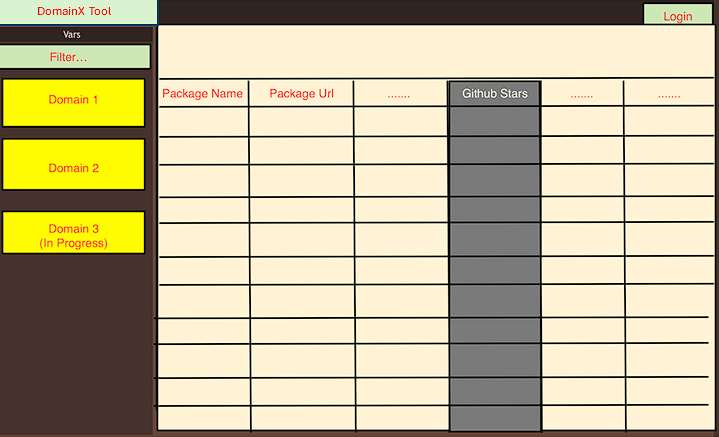
\includegraphics[totalheight=8cm]{images/DomainX-UI.png}
  \caption{DomainX UI, inspired by Octave Online}
  \label{fig:domainx_ui}
\end{figure}
\newpage{}
\section*{Appendix --- Reflection}

The purpose of reflection questions is to give you a chance to assess your own
learning and that of your group as a whole, and to find ways to improve in the
future. Reflection is an important part of the learning process.  Reflection is
also an essential component of a successful software development process.  

Reflections are most interesting and useful when they're honest, even if the
stories they tell are imperfect. You will be marked based on your depth of
thought and analysis, and not based on the content of the reflections
themselves. Thus, for full marks we encourage you to answer openly and honestly
and to avoid simply writing ``what you think the evaluator wants to hear.''

Please answer the following questions.  Some questions can be answered on the
team level, but where appropriate, each team member should write their own
response:


\begin{enumerate}
  \item What went well while writing this deliverable? 
  \item What pain points did you experience during this deliverable, and how did
  you resolve them?
  \item How many of your requirements were inspired by speaking to your
  client(s) or their proxies (e.g. your peers, stakeholders, potential users)?
  \item Which of the courses you have taken, or are currently taking, will help
  your team to be successful with your capstone project.
  \item What knowledge and skills will the team collectively need to acquire to
  successfully complete this capstone project?  Examples of possible knowledge
  to acquire include domain specific knowledge from the domain of your
  application, or software engineering knowledge, mechatronics knowledge or
  computer science knowledge.  Skills may be related to technology, or writing,
  or presentation, or team management, etc.  You should look to identify at
  least one item for each team member.
  \item For each of the knowledge areas and skills identified in the previous
  question, what are at least two approaches to acquiring the knowledge or
  mastering the skill?  Of the identified approaches, which will each team
  member pursue, and why did they make this choice?
\end{enumerate}


\end{document}